\documentclass[full-course-notes.tex]{subfiles}

\begin{document}
\lecturemeta{2}
  {Structure of a Compiler: Phases Overview; Front-/Middle-/Back-End; MLIR and Real-World IRs}
  {CLO 1}
  {\S1.2 (The Structure of a Compiler), \S2.1--\S2.8 (overview of a syntax-directed translator's stages)}
  {[PP] Programming Language Pragmatics \S1.5, \S1.6}
\lecshort{Structure of a Compiler}
\setcounter{section}{0}
\makelecturetitle

\begin{coreidea}[Lecture Roadmap]
\begin{enumerate}
  \item The classical phase pipeline of a compiler (DB Fig.\,1.6): what each phase consumes and
  produces, followed all the way through on one tiny worked example.
  \item The two cross-cutting components every phase touches: the \textbf{symbol table} and
  \textbf{error handling}.
  \item Grouping the phases into \textbf{front-end / middle-end / back-end}, and why that
  grouping is an engineering decision, not just a diagram convenience.
  \item How real-world intermediate representations -- \textbf{LLVM IR, JVM bytecode,
  WebAssembly, and MLIR} -- relate to this pipeline and to each other.
\end{enumerate}
Today is still ``the outside view.'' From Lecture~\ref{lec:3} onward we go phase-by-phase in
depth, starting with lexical analysis. (The preprocessor/assembler/linker/loader toolchain
around the compiler was already covered in Lecture~\ref{lec:1}.)
\end{coreidea}

\section{The Phase Pipeline of a Compiler}
\label{sec:l2-phase-pipeline}

\dbtag DB organizes a compiler as a pipeline of phases, each of which takes the output of the
previous phase as input, checks it, and produces a new representation of the program one step
closer to executable code.

\begin{center}
\begin{tikzpicture}[
  ph/.style={draw, thick, rounded corners, minimum height=0.8cm, minimum width=6.5cm, align=center, font=\bfseries\small},
  fe/.style={ph, fill=dbGreenBg, draw=dbGreen},
  mid/.style={ph, fill=enrichGoldBg, draw=enrichGold},
  be/.style={ph, fill=examRedBg, draw=examRed},
  node distance=0.4cm
]
  \node[fe] (lex) {Lexical Analysis (Scanning)};
  \node[fe, below=of lex] (syn) {Syntax Analysis (Parsing)};
  \node[fe, below=of syn] (sem) {Semantic Analysis};
  \node[mid, below=of sem] (icg) {Intermediate Code Generation};
  \node[mid, below=of icg] (opt) {Machine-Independent Code Optimization};
  \node[be, below=of opt] (cg) {Code Generation};
  \node[be, below=of cg] (mopt) {Machine-Dependent Code Optimization};

  \foreach \a/\b in {lex/syn, syn/sem, sem/icg, icg/opt, opt/cg, cg/mopt}
    \draw[-{Latex[length=3mm]}, thick] (\a) -- (\b);
\end{tikzpicture}
\end{center}

\begin{center}
\renewcommand{\arraystretch}{1.3}
\begin{tabularx}{\textwidth}{@{}l l X@{}}
\toprule
\textbf{Phase} & \textbf{Input} & \textbf{Output} \\
\midrule
Lexical Analysis & Raw character stream & Stream of \textbf{tokens} (e.g.\ \texttt{ID}, \texttt{NUM}, \texttt{+}) \\
Syntax Analysis & Token stream & \textbf{Syntax tree} (or parse tree) capturing grammatical structure \\
Semantic Analysis & Syntax tree & Annotated (``decorated'') tree: types checked, scopes resolved \\
Intermediate Code Gen. & Annotated tree & Machine-independent \textbf{IR}, e.g.\ three-address code \\
Code Optimization & IR & Improved, semantically-equivalent IR \\
Code Generation & Optimized IR & Target-machine code (often assembly) \\
\bottomrule
\end{tabularx}
\end{center}

\begin{examfocus}
Memorize the phase order and, for each phase, one sentence describing its input and output.
This exact table (input $\to$ phase $\to$ output) is the single most common short-answer /
MCQ pattern in compiler exams worldwide, not just here.
\end{examfocus}

\subsection{A Tiny Example, Followed Through Every Phase}
\label{sec:l2-tiny-example}

\dbtag It helps enormously to see one small piece of source code survive the \emph{entire}
pipeline, phase by phase, before we study each phase in isolation over the coming lectures. DB
uses exactly this running example when it first introduces the phases (\S1.2); we reproduce a
miniature version of it here, and will point back to it by name (``the \texttt{position}
example'') whenever a later lecture revisits one of these phases in more depth. Nothing here
needs to be memorized yet -- it is a preview, not new material to be tested on its own.

Source statement (assume \texttt{position}, \texttt{initial}, and \texttt{rate} are declared as
real/floating-point variables, and \texttt{60} is an ordinary integer literal):
\begin{center}
\ttfamily position = initial + rate * 60
\end{center}

\begin{defbox}{Token and Lexeme}
A \textbf{lexeme} is the actual sequence of characters in the source program that the lexical
analyzer recognizes as a single meaningful unit -- for example, the seven characters
\texttt{p-o-s-i-t-i-o-n} form one lexeme, and the single character \texttt{=} forms another. A
\textbf{token} is the abstract \texttt{<token-name, attribute-value>} pair the lexer emits once
it has recognized a lexeme: the token-name records \emph{which category} was matched (e.g.\
\texttt{ID}, \texttt{ASSIGN}, \texttt{PLUS}), and the attribute-value carries whatever extra
information later phases need in order to tell this particular lexeme apart from other lexemes
in the same category -- for an identifier, almost always a pointer into the symbol table.
Lecture~\ref{lec:3} gives the full formal treatment, including \textbf{patterns} -- the rules
that describe which lexemes belong to which token.
\end{defbox}

For this statement, the \textbf{lexemes} are the individual pieces of source text
\texttt{position}, \texttt{=}, \texttt{initial}, \texttt{+}, \texttt{rate}, \texttt{*}, and
\texttt{60}. Lexical analysis classifies each one as a \textbf{token}: the lexeme
\texttt{position} becomes \texttt{<ID, ptr to symtab entry for \texttt{position}>} -- written
\texttt{<id,1>} in the walkthrough below -- and likewise \texttt{initial} and \texttt{rate}
become \texttt{<id,2>} and \texttt{<id,3>}; the lexeme \texttt{=} becomes an
\texttt{<ASSIGN>} token, \texttt{+} a \texttt{<PLUS>} token, \texttt{*} a \texttt{<MULT>} token,
and \texttt{60} a \texttt{<NUM, 60>} token. None of the three operator tokens need an
attribute-value, since the token-name alone already tells the parser everything it needs to
know.

\begin{examplebox}{The \texttt{position} Statement, Phase by Phase}
\begin{itemize}
  \item \textbf{Lexical analysis (Lectures 3--7).} The character stream is grouped into tokens:
  \texttt{<id,1> <=> <id,2> <+> <id,3> <*> <60>} -- where \texttt{id,1}, \texttt{id,2}, and
  \texttt{id,3} are pointers to the symbol-table entries for \texttt{position}, \texttt{initial},
  and \texttt{rate} respectively.
  \item \textbf{Syntax analysis (Lectures 8--17).} The token stream is organized into a syntax
  tree that reflects the grammatical structure of an assignment: an \texttt{=} node whose left
  child is \texttt{id,1} and whose right child is a \texttt{+} node, which in turn has children
  \texttt{id,2} and a \texttt{*} node with children \texttt{id,3} and \texttt{60}.
  \item \textbf{Semantic analysis (Lectures 18--21).} Types are checked, and where necessary,
  made explicit. Here, \texttt{60} is an integer literal but \texttt{rate} is real, so the
  semantic analyzer inserts an explicit conversion: the \texttt{*} node's right child becomes
  \texttt{inttoreal(60)} instead of the bare integer \texttt{60}. The result is an
  \emph{annotated} (``decorated'') tree.
  \item \textbf{Intermediate code generation (Lectures 22--25).} The annotated tree is
  translated into three-address code, one operation per instruction:
\begin{verbatim}
t1 = inttoreal(60)
t2 = id3 * t1
t3 = id2 + t2
id1 = t3
\end{verbatim}
  \item \textbf{Code optimization (Lectures 28--29).} \texttt{inttoreal(60)} does not depend on
  any variable, so it can be computed once, at compile time, instead of being recomputed by the
  generated program every single time this line runs:
\begin{verbatim}
t1 = id3 * 60.0
id1 = id2 + t1
\end{verbatim}
  \item \textbf{Code generation (Lecture 30).} The optimized IR becomes target assembly, using
  real machine registers and instructions (illustrative syntax, not tied to one specific ISA):
\begin{verbatim}
MOVF   id3, R2
MULF   #60.0, R2
MOVF   id2, R1
ADDF   R2, R1
MOVF   R1, id1
\end{verbatim}
\end{itemize}
\end{examplebox}

The syntax-analysis step above builds the following syntax tree -- the root \texttt{=} node
assigns to \texttt{id,1} the value computed by its right subtree:

\begin{center}
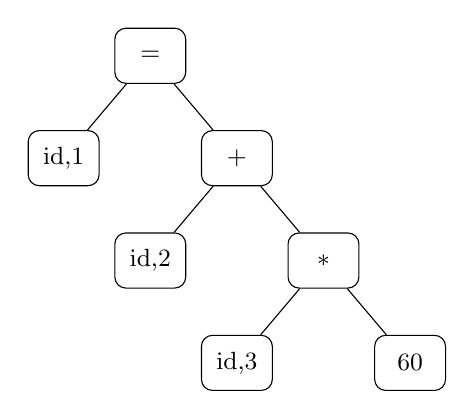
\begin{tikzpicture}[
  level distance=13mm,
  sibling distance=22mm,
  every node/.style={draw, rounded corners, minimum width=9mm, minimum height=7mm, align=center, font=\small}
]
\node {=}
  child { node {id,1} }
  child { node {+}
    child { node {id,2} }
    child { node {$*$}
      child { node {id,3} }
      child { node {60} }
    }
  }
;
\end{tikzpicture}
\end{center}
\begin{center}
\small\textit{Syntax tree for \texttt{position = initial + rate * 60}.}
\end{center}

\begin{examfocus}
This example is deliberately small enough to hold in your head. When a later lecture introduces
the \emph{real} algorithm for a phase (Thompson's construction, LALR(1) table construction,
available-expressions data-flow analysis, and so on), try re-running that algorithm on this same
statement by hand before tackling a harder one -- it is a fast way to sanity-check that you have
understood a new algorithm correctly.
\end{examfocus}

\subsection{Analysis and Synthesis: The Two Halves}
\label{sec:l2-analysis-synthesis}

\dbtag DB groups these six phases into two conceptual halves:

\begin{itemize}
  \item \textbf{Analysis part (``front end''):} lexical, syntax, and semantic analysis, plus
  intermediate code generation. This half \emph{breaks down} the source program and builds an
  intermediate representation plus a record of the program's structure (the symbol table).
  Analysis is where most \textbf{compile-time errors} are caught and reported.
  \item \textbf{Synthesis part (``back end''):} optimization and code generation. This half
  \emph{constructs} the desired target program from the intermediate representation and symbol
  table.
\end{itemize}

\begin{defbox}{Analysis-Synthesis Model}
A compiler can be understood as consisting of an \textbf{analysis} part, which breaks the
source program into pieces and builds an intermediate representation, and a \textbf{synthesis}
part, which constructs the target program from that intermediate representation. This is DB's
own high-level characterization of \emph{every} compiler, regardless of source or target
language.
\end{defbox}

\section{Symbol Table and Error Handling: The Cross-Cutting Phases}
\label{sec:l2-symtab-error}

\dbtag Two components are not steps in the pipeline --- they run \emph{alongside every phase},
being read from and written to throughout the whole compilation: the \textbf{symbol table} and
\textbf{error handling}.

\begin{defbox}{Symbol Table}
A \textbf{symbol table} is a data structure that records every identifier declared in a program
-- variables, function names, class names -- together with the attributes later phases need to
know about it: its \textbf{type}, \textbf{scope}, \textbf{memory location}, and, for functions,
its parameter and return types. It is not itself one of the six phases; instead every phase
reads from it and writes to it: lexical analysis creates an entry the first time it sees a new
identifier, semantic analysis fills in type information once it is known, and code generation
consults it to compute final memory addresses.
\end{defbox}

\begin{examplebox}{Symbol Table Contents for the \texttt{position} Example}
For \texttt{position = initial + rate * 60} (\Sref{sec:l2-tiny-example}), lexical analysis
creates one entry per distinct identifier -- exactly the \texttt{id,1}, \texttt{id,2}, and
\texttt{id,3} pointers used throughout that walkthrough:
\begin{center}
\renewcommand{\arraystretch}{1.3}
\begin{tabularx}{\textwidth}{@{}l l l X@{}}
\toprule
\textbf{Entry} & \textbf{Name} & \textbf{Type} & \textbf{Role in this statement} \\
\midrule
\texttt{id,1} & \texttt{position} & real & assigned to \\
\texttt{id,2} & \texttt{initial} & real & read \\
\texttt{id,3} & \texttt{rate} & real & read \\
\bottomrule
\end{tabularx}
\end{center}
Notice \texttt{60} never gets its own entry -- it is a numeric \emph{literal}, not an
identifier, so it is carried as a token attribute (\texttt{<NUM, 60>}) rather than being
recorded in the symbol table.
\end{examplebox}

\textbf{Error handling.} Each phase may encounter errors specific to its own level: lexical
analysis catches malformed tokens, syntax analysis catches grammatically invalid programs,
semantic analysis catches type mismatches and undeclared identifiers. A well-built compiler
tries to \emph{recover} from an error and keep going, so it can report several distinct errors
from a single compilation run instead of stopping at the first one.

\subsection{Lexical, Syntax, and Semantic Errors}
\label{sec:l2-error-kinds}

\dbtag The three kinds of errors above are easy to name but easy to blur together in practice.
Getting the distinction right matters because it tells you \emph{which phase} is responsible for
catching a given mistake -- and, just as importantly, which phases are \emph{not} responsible
for it and will happily let it through.

\begin{defbox}{Lexical, Syntax, and Semantic Errors}
\begin{itemize}
  \item A \textbf{lexical error} occurs when the lexer meets a character sequence that matches
  \emph{no pattern for any token at all} -- e.g.\ an illegal character, an unterminated string
  or comment, or a malformed numeric literal. The lexer fails before the parser ever sees this
  part of the input.
  \item A \textbf{syntax error} occurs when the token stream -- with every individual token
  itself perfectly valid -- does not conform to the grammar: e.g.\ a missing semicolon, an
  unbalanced parenthesis, or an operator with no right-hand operand.
  \item A \textbf{semantic error} occurs when the program is grammatically well formed but
  violates a rule about \emph{meaning} that the language enforces: e.g.\ using an undeclared
  identifier, assigning incompatible types, or calling a function with the wrong number of
  arguments.
\end{itemize}
Each is caught by a different phase, in this order, because each phase can only see what the
phase before it has already built: lexical analysis sees individual characters, syntax analysis
sees the shape of the token stream, and semantic analysis is the first phase that understands
what the program actually \emph{means} (using the symbol table above to check declarations,
types, and scope).
\end{defbox}

\begin{examplebox}{One Error of Each Kind, in One Function}
\begin{verbatim}
int main() {
    int count = 0;
    int limit = 10           /* (1) */

    while (count < limit) {
        count = count # 1;   /* (2) */
        total = total + count;   /* (3) */
    }

    printf("Final count = %d", count);
    return 0;
}
\end{verbatim}
\begin{center}
\renewcommand{\arraystretch}{1.3}
\begin{tabularx}{\textwidth}{@{}l l X@{}}
\toprule
\textbf{Line} & \textbf{Error Kind} & \textbf{Why} \\
\midrule
(1) & Syntax & \texttt{int limit = 10} is missing the terminating \texttt{;}. Every token on
this line is individually a valid token -- the parser is the one that fails, because it cannot
complete the grammar rule for a declaration statement without a semicolon before the next
statement begins. \\
(2) & Lexical & \texttt{\#} is not a valid character inside a C expression. No token pattern
matches it at all, so the \emph{lexer itself} fails right here -- the parser never even gets a
chance to see this line. \\
(3) & Semantic & \texttt{total} is used but was never declared anywhere in this function. Every
token is valid and the statement is a grammatically perfect assignment, so only semantic
analysis -- which checks the symbol table for declarations and scope -- can catch this. \\
\bottomrule
\end{tabularx}
\end{center}
Notice the ordering this implies: if line (2)'s illegal character were fixed but line (1)'s
missing semicolon were not, the compiler would still stop at the syntax error before ever
reaching semantic analysis and reporting the undeclared \texttt{total} on line (3) -- each phase
only gets to run once the phase before it has accepted its input.
\end{examplebox}

\begin{examfocus}
Given a short, broken code snippet, be able to classify each mistake as lexical, syntax, or
semantic, and justify the classification the way the table above does -- this is one of the most
common short-answer formats for this topic. A frequent trap: a misspelled \emph{keyword} (like
\texttt{fi} for \texttt{if}) is \textbf{not} a lexical error, because it is still a perfectly
valid lexeme for token \texttt{ID} -- the mistake only surfaces later, as a syntax error (if
\texttt{fi} appears somewhere no identifier is grammatically valid) or a semantic error (if it is
used as if it were a declared function or variable).
\end{examfocus}

\begin{center}
\resizebox{0.85\textwidth}{!}{%
\begin{tikzpicture}[
  ph/.style={draw, thick, rounded corners, minimum height=0.85cm, minimum width=3.6cm, align=center, fill=nuLight, draw=nuNavy, font=\small},
  side/.style={draw, thick, rounded corners, minimum height=4.9cm, minimum width=2.6cm, align=center, font=\small\bfseries, text width=2.3cm},
  node distance=0.4cm
]
  \node[ph] (lex) {Lexical Analysis};
  \node[ph, below=of lex] (syn) {Syntax Analysis};
  \node[ph, below=of syn] (sem) {Semantic Analysis};
  \node[ph, below=of sem] (icg) {Interm.\ Code Gen};
  \node[ph, below=of icg] (cg) {Code Generation};
  \foreach \a/\b in {lex/syn, syn/sem, sem/icg, icg/cg}
    \draw[-{Latex[length=2.5mm]}, thick] (\a) -- (\b);

  \node[side, fill=takeawayTealBg, draw=takeawayTeal, left=1.6cm of syn, yshift=-1.1cm] (st) {Symbol Table};
  \node[side, fill=examRedBg, draw=examRed, right=1.6cm of syn, yshift=-1.1cm] (eh) {Error Handler};

  \foreach \p in {lex, syn, sem, icg, cg}{
    \draw[-{Latex[length=2mm]}, gray, dashed] (\p.west) -- (st.east |- \p.west);
    \draw[-{Latex[length=2mm]}, gray, dashed] (\p.east) -- (eh.west |- \p.east);
  }
\end{tikzpicture}}
\end{center}

\begin{enrichment}[Extra Depth: What Real Symbol Tables Store]
A production compiler's symbol table stores far more than DB's introductory description
suggests: mangled names (for overload resolution in C++/Rust), calling-convention information,
alignment and padding requirements, visibility/linkage (\texttt{static} vs.\ exported), inlining
hints, and --- in languages with generics/templates --- a separate table per instantiation.
Modern compilers often implement it not as one flat table but as a \textbf{chain of nested
scopes} (a scope stack or scope tree), so that entering a block, function, or class pushes a
new scope that shadows outer ones and is popped on exit. LLVM's \texttt{clang} keeps this
information in its \texttt{Decl} hierarchy rather than a single table, reflecting how much richer
real symbol-table designs are compared to the simple table DB introduces.
\end{enrichment}

\section{Grouping the Phases: Front-End, Middle-End, Back-End}
\label{sec:l2-grouping-phases}

\beyonddb DB's own diagram groups phases into analysis/synthesis, but the vocabulary you will
hear constantly in industry and in later lectures is \textbf{front-end / middle-end / back-end}.
This is not just relabeling --- it reflects a real engineering strategy.

\begin{center}
\renewcommand{\arraystretch}{1.3}
\begin{tabularx}{\textwidth}{@{}l X@{}}
\toprule
\textbf{Group} & \textbf{Contains / Responsibility} \\
\midrule
\textbf{Front-end} & Lexical, syntax, semantic analysis. Language-\emph{specific}: knows the
grammar and type rules of exactly one source language, and lowers it to a common IR. \\
\textbf{Middle-end} & Machine-independent optimization on the IR. Language-\emph{agnostic} and
target-\emph{agnostic}: the same optimization passes (constant folding, dead-code elimination,
inlining) apply no matter which source language or target CPU is involved. \\
\textbf{Back-end} & Code generation and machine-dependent optimization. Target-\emph{specific}:
knows the instruction set, register file, and calling convention of exactly one target
architecture. \\
\bottomrule
\end{tabularx}
\end{center}

\begin{coreidea}[Why This Grouping Is the Whole Point]
If front-ends only ever talk to a shared IR, and back-ends only ever talk to that same shared
IR, then supporting a new \emph{source language} only requires writing one new front-end --- it
automatically gets every optimization and every target the IR already supports. Symmetrically,
supporting a new \emph{target CPU} only requires writing one new back-end --- it automatically
works for every source language already supported. Without this split, you would need to write a
separate optimizer and code generator for every (language, target) \emph{pair} --- the classic
``$M$ languages $\times$ $N$ targets'' problem, needing on the order of $M \times N$ components
instead of $M + N$.
\end{coreidea}

\begin{historynote}
This $M \times N$ argument predates LLVM by decades. In the 1960s, \textbf{T-diagrams}
(popularized by F.\,L.\ Bauer and others) were a standard notation for exactly this problem:
a T-shaped diagram showing a compiler written in language $H$, translating source language $S$
into target language $T$. Compiler writers used T-diagrams to reason about \emph{bootstrapping}
(compiling a new compiler using an existing one) and about how many compilers you actually need
to support $M$ languages on $N$ machines --- precisely the front-end/back-end decoupling
argument above, expressed sixty years earlier with pen-and-paper diagrams instead of shared IR
software.
\end{historynote}

\begin{enrichment}[Extra Depth: The Front/Middle/Back Split in a Real Toolchain --- LLVM]
The clearest concrete instance of this architecture today is LLVM, and it is worth walking
through once here since we will return to it in Lecture 25 for code generation proper.
\begin{itemize}
  \item \textbf{Front-end (Clang, for C/C++/Objective-C):} lexes and parses source into a
  Clang-specific Abstract Syntax Tree (AST), performs semantic analysis and type checking on
  that AST, then \emph{lowers} it into \textbf{LLVM IR} --- a typed, SSA-based (Static Single
  Assignment) intermediate representation that is completely independent of C++ as a language.
  Rust (\texttt{rustc}), Swift, Julia, and Zig all have their own, completely different
  front-ends, but they all emit the \emph{same} LLVM IR.
  \item \textbf{Middle-end (the LLVM optimizer, \texttt{opt}):} a pipeline of dozens of
  independent \textbf{passes} --- e.g.\ \texttt{mem2reg} (promote stack variables to SSA
  registers), \texttt{instcombine} (peephole-simplify instruction sequences),
  \texttt{inline} (function inlining), \texttt{gvn} (global value numbering, subsuming common
  subexpression elimination), \texttt{loop-vectorize} --- each of which reads LLVM IR and
  produces improved LLVM IR. None of these passes know or care whether the original source was
  C++, Rust, or Swift.
  \item \textbf{Back-end (\texttt{llc}, or the integrated code generator):} lowers optimized
  LLVM IR to a specific target's machine code --- x86-64, AArch64, RISC-V, or even WebAssembly,
  selected via a \texttt{-target} triple. Instruction selection, register allocation, and
  instruction scheduling all happen here, specific to that one target.
\end{itemize}
The practical payoff: when Apple Silicon (AArch64) needed a good C++ compiler, no one had to
write a new C++ front-end --- Clang's C++ front-end and every middle-end optimization pass were
already reusable; only a back-end for AArch64 was needed (and it mostly already existed, since
LLVM had supported ARM for years). This is exactly the $M+N$ payoff from the coreidea box above,
made concrete: roughly 20+ front-ends (Clang, \texttt{rustc}, Swift, Julia, \dots) and roughly
20+ back-ends (x86-64, AArch64, RISC-V, WebAssembly, \dots) share \emph{one} middle-end, instead
of each of those $20 \times 20$ combinations needing its own hand-written optimizer.
\end{enrichment}

\begin{enrichment}[Extra Depth: The Front-End's Second Career --- IDEs and Language Servers]
The front-end (lexer + parser + semantic analyzer) is valuable even when no target code is ever
generated. This observation underlies the \textbf{Language Server Protocol (LSP)}: an editor
like VS Code or Neovim talks to a background process (a ``language server'') that re-runs a
language's front-end on every keystroke to provide autocomplete, jump-to-definition, and
real-time error squiggles --- all without ever reaching code generation. \texttt{clangd} (built
directly on Clang's front-end), \texttt{rust-analyzer}, and \texttt{gopls} are all, in effect,
``compilers with the back end removed and an editor bolted on instead.'' This is a direct,
practical payoff of the front-end/back-end separation described above: a front-end built for
compilation can be repurposed wholesale for tooling.
\end{enrichment}

\section{Comparing Real-World IRs: LLVM IR, JVM Bytecode, and WebAssembly}
\label{sec:l2-ir-comparison}

\beyonddb LLVM IR, JVM bytecode, and WebAssembly are all, loosely, ``intermediate,
machine-independent instruction sets sitting between source code and a real CPU'' --- which is
why students often lump them together as interchangeable ``bytecode.'' They are not
interchangeable: each was designed with a different primary goal in mind, and that goal shapes
how high- or low-level it is, what it assumes about memory and objects, and what it is actually
good for.

\begin{center}
\renewcommand{\arraystretch}{1.5}
\small
\begin{tabularx}{\textwidth}{@{}l X X X@{}}
\toprule
 & \textbf{LLVM IR} & \textbf{JVM Bytecode} & \textbf{WebAssembly (Wasm)} \\
\midrule
\textbf{Primary design goal} & A reusable \emph{compiler middle-end}: one optimizer, shared by
many front-ends and back-ends & \emph{Portability} (``write once, run anywhere'') for
Java-family, object-oriented, garbage-collected languages & \emph{Safe, sandboxed} execution of
code from an untrusted source (originally: the web), at near-native speed \\
\textbf{Abstraction level} & Low --- close to assembly, but target-independent; typed and
SSA-based & Medium-to-high --- bakes in classes, interfaces, virtual method dispatch, exception
tables & Low --- a compact, portable, stack-based instruction set, close to assembly \\
\textbf{Assumes an object model / GC?} & No. No built-in notion of classes or garbage
collection; each front-end supplies its own & Yes. Assumes the JVM supplies garbage collection
and an object model & No, in Wasm's core spec. A separate, later ``GC proposal'' adds optional
managed references \\
\textbf{Control flow} & Ordinary basic blocks and branches, the same shape as real machine code
& Ordinary jumps/branches; the bytecode \emph{verifier} checks type-safety, not control-flow
shape & \textbf{Structured only} --- blocks, loops, ifs; no arbitrary \texttt{goto}, so a
validator can check it in a single linear pass \\
\textbf{Usually executed directly?} & No --- almost always compiled further, to native code; not
normally shipped as the final artifact users run & Yes --- interpreted and/or JIT-compiled
directly by a JVM & Yes --- interpreted and/or JIT/AOT-compiled directly by a Wasm runtime \\
\textbf{Best fit for} & Being a shared layer that \emph{very different} source languages
(systems, functional, managed, \dots) can all lower into & Languages that already fit the JVM's
object/GC model well (Kotlin, Scala, Clojure, Groovy) & Any source language willing to compile
to a small, safe, sandboxed core -- often reached \emph{via} LLVM's own WebAssembly back-end \\
\bottomrule
\end{tabularx}
\end{center}

\begin{coreidea}[Why LLVM IR's Low Level Is a Feature, Not a Limitation]
LLVM IR deliberately does \emph{not} assume any particular memory-management strategy or object
model. That is exactly why it can serve as the shared middle layer for languages with wildly
different runtime models: C's manual memory management, Rust's ownership/borrow-checked memory,
Swift's automatic reference counting, and Julia's dynamic dispatch all lower into the same LLVM
IR, because none of those choices had to be baked into the IR itself -- each front-end encodes
its own memory-management decisions \emph{as ordinary LLVM IR instructions}. JVM bytecode makes
the opposite trade-off: by assuming garbage collection and an object model up front, it becomes
an excellent, low-friction target for languages that already want exactly that (Kotlin, Scala)
but an awkward one for a language like C that manages memory itself. Neither design is
``better'' in general -- they optimize for different things, which is precisely the point of
this comparison.
\end{coreidea}

\begin{examplebox}{WebAssembly as ``Just Another LLVM Back-End''}
Because LLVM already has back-ends for x86-64, AArch64, and RISC-V, adding a WebAssembly
back-end fits the exact same $M+N$ story from earlier in this lecture: any existing LLVM
front-end (Clang for C/C++, \texttt{rustc} for Rust) can already produce WebAssembly simply by
selecting the \texttt{wasm32} target, with \emph{no} changes to the front-end or to any
optimization pass. This is why, in practice, a great deal of WebAssembly in the wild is not
hand-written but is the output of compiling C, C++, or Rust source through ordinary LLVM
tooling (e.g.\ Emscripten for C/C++) -- WebAssembly is simultaneously a stand-alone IR in its own
right \emph{and} one more entry in LLVM's list of back-end targets.
\end{examplebox}

\begin{examfocus}
Do not confuse the two axes this section and the earlier ``kinds of IR'' discussion test
separately: \emph{how low-level is it, and why} (this section) versus \emph{when is it executed
relative to run time} (Lecture~\ref{lec:1}'s AOT/interpreter/JIT distinction). LLVM IR and WebAssembly are
both low-level, but for different reasons -- LLVM IR is low-level so that generating real machine
code from it is easy and so that no language's runtime assumptions get baked in; WebAssembly is
low-level \emph{and} structured so that it can be validated quickly and executed safely in a
sandbox. JVM bytecode is higher-level than both, by design, because portability for one specific
family of managed languages -- not raw compiler-infrastructure reuse, and not sandboxed safety
for arbitrary source languages -- was its original goal.
\end{examfocus}

\section{MLIR: A Framework for Building Compiler IRs}
\label{sec:l2-mlir}

MLIR (``Multi-Level Intermediate Representation'') is a compiler-infrastructure project started
at Google around 2019 and merged into the official LLVM monorepo as one of its sub-projects in
2020, first described publicly in~\cite{mlir}. It is worth understanding alongside LLVM IR for the same reason the
previous section compared LLVM IR, JVM bytecode, and WebAssembly: people often assume ``MLIR''
is just another name for ``LLVM IR, but newer,'' when in fact the two solve different problems
and sit at different points in a compiler's pipeline.

\subsection{The Problem MLIR Was Built to Solve}
\label{sec:l2-mlir-problem}

LLVM IR is deliberately low-level: typed, in SSA form, organized into ordinary basic blocks --
close to assembly, as \Sref{sec:l2-ir-comparison} described. That is exactly what makes it a good shared target for many
different \emph{source} languages once they have already been reduced to simple operations and
control flow. It is a poor fit, however, for representing a program \emph{before} that
reduction has happened -- for example, a matrix multiplication expressed as a single high-level
tensor operation, or a nested loop that a compiler still intends to tile, fuse, or vectorize as a
unit. Lowering straight to LLVM IR forces that structure to be flattened away immediately, before
any optimization pass gets a chance to use it.

Before MLIR existed, projects that needed this kind of higher-level representation simply built
their own IR from scratch: TensorFlow's XLA had its own IR for tensor computations, Swift had
SIL, Rust had MIR, and so on. Each of these reimplemented the same underlying machinery --
a verifier, a textual printer and parser, a pass manager, a way to track source locations for
error messages -- that LLVM already provides for LLVM IR, but for their own, unrelated IR. MLIR's
goal is to give every such project a shared framework for this machinery, so that building a new,
domain-specific IR is a matter of defining new operations rather than rebuilding compiler
infrastructure from the ground up.

\subsection{Core Ideas}
\label{sec:l2-mlir-core-ideas}

\textbf{Dialects.} Instead of one fixed instruction set, MLIR defines an extensible mechanism
for registering \textbf{dialects} -- namespaced families of operations, types, and attributes.
The \texttt{arith} dialect has operations like \texttt{arith.addi}; the \texttt{linalg} dialect
has structured, high-level operations such as matrix multiplication; the \texttt{scf} dialect
(``structured control flow'') has \texttt{for} and \texttt{while} loops as single operations,
rather than as jumps between basic blocks; and the \texttt{llvm} dialect defines operations that
directly mirror LLVM IR. Crucially, operations from several different dialects can appear
together in the very same function -- there is no requirement to fully translate out of one
dialect before using another.

\textbf{Progressive lowering.} A program does not jump from a high-level dialect straight to
machine code in one step. It is lowered dialect by dialect: a high-level tensor operation
becomes a structured loop, the structured loop becomes ordinary branching control flow, and
that, in turn, becomes the \texttt{llvm} dialect. Each of these steps is a small, independently
checkable transformation, and different compilers can choose to stop lowering at whichever level
is most useful for a given optimization -- a loop-tiling pass wants to run before loops are
flattened into branches, for instance, while register allocation only makes sense long after
that point.

\textbf{Regions.} An ordinary LLVM IR function is a flat sequence of basic blocks connected by
branches -- there is no notion of one block being ``inside'' another. An MLIR operation, by
contrast, can carry a nested \textbf{region} containing its own blocks. A loop or a function body
is therefore naturally represented as one operation containing a region, preserving its nested
structure for as long as that structure remains useful, instead of being flattened into a
control-flow graph immediately.

\subsection{How MLIR Differs From LLVM IR}
\label{sec:l2-mlir-vs-llvm}

\begin{center}
\renewcommand{\arraystretch}{1.4}
\begin{tabularx}{\textwidth}{@{}l X X@{}}
\toprule
 & \textbf{LLVM IR} & \textbf{MLIR} \\
\midrule
What it is & One fixed intermediate representation & A framework for defining many
intermediate representations (dialects) \\
Abstraction level & Low and fixed -- close to assembly & Whatever a given dialect needs --
high, low, or several levels mixed in one module \\
Control-flow structure & Flat basic blocks connected by branches & Operations can carry nested
regions, so loops and other structure can stay nested until a pass chooses to flatten them \\
Role in a pipeline & The representation code is lowered \emph{to}, immediately before
LLVM's own optimizer and back-ends take over & Sits \emph{upstream} of LLVM IR; its own
\texttt{llvm} dialect is what eventually converts into ordinary LLVM IR \\
\bottomrule
\end{tabularx}
\end{center}

The last row is the point most often missed: MLIR does not replace LLVM. A program written using
MLIR's higher-level dialects is progressively lowered, within MLIR, down to the \texttt{llvm}
dialect; from there it is translated into ordinary LLVM IR and handed to the exact same
optimizer passes and back-ends already described in \Sref{sec:l2-grouping-phases} and
\Sref{sec:l2-ir-comparison}. MLIR extends the \emph{front}
of the pipeline -- giving compiler writers a place to do domain-specific reasoning (tensor
shapes, loop tiling, hardware-specific fusion) before code is flattened down to LLVM IR -- rather
than replacing anything downstream of it.

\subsection{Where MLIR Is Used}
\label{sec:l2-mlir-adopters}

MLIR's dialect mechanism has made it attractive well beyond its original use case. Notable
adopters include Google's XLA and IREE (compiling machine-learning computation graphs to CPUs,
GPUs, and custom accelerators), PyTorch's Torch-MLIR, Triton (a language for writing GPU
kernels), CIRCT (an MLIR-based toolchain for hardware design, playing a role similar to parts of
a Verilog toolchain), and Flang, LLVM's own Fortran front end, which lowers through an
MLIR dialect called FIR before reaching LLVM IR (see \cite{mlir,mlirdocs} for further reading).

\section{Self-Check Questions}
\label{sec:l2-selfcheck}

\begin{enrichment}[Practice -- Not Graded]
\begin{enumerate}
  \item Place the following in correct pipeline order: semantic analysis, linking, assembly,
  lexical analysis, loading, syntax analysis, preprocessing, code generation.
  \item A program calls a function defined in a library it never \texttt{\#include}s a
  declaration for, but the linker still resolves the call successfully because the symbol name
  matches at link time. Which phase would have caught this as an error if the declaration truly
  were missing, and why didn't it?
  \item Explain, in the M-languages/N-targets argument, why a shared IR turns an
  $M \times N$ problem into an $M + N$ problem. What is the "shared IR" in LLVM's case?
  \item Why does dynamic linking trade smaller executables for slower startup, while static
  linking does the opposite?
  \item \texttt{clangd} never performs code generation. Which phases of the pipeline does it
  still need to run, and why are those enough to power features like ``jump to definition''?
  \item For the \texttt{position} example in \Sref{sec:l2-tiny-example}, write out what the three-address code would
  look like if \texttt{60} were replaced by \texttt{count}, an already-integer variable (so no
  \texttt{inttoreal} conversion is needed). Which of the six phases changes as a result, and
  which stay exactly the same?
  \item JVM bytecode assumes garbage collection; LLVM IR does not. Explain why this makes JVM
  bytecode a natural fit for Kotlin but a poor natural fit for a language like C, and explain why
  WebAssembly's core spec makes the same choice as LLVM IR here rather than the JVM's.
  \item For the statement \texttt{count = count + step}, list its lexemes, give the
  \texttt{<token-name, attribute-value>} pair for each one, and sketch the symbol table entries
  lexical analysis would create (assuming \texttt{count} and \texttt{step} are both integers).
  \item Draw the syntax tree for \texttt{count = count + step} in the same style as the
  \texttt{position} example's tree, and identify which single node the semantic analyzer would
  need to annotate if \texttt{step} were declared \texttt{real} instead of integer.
  \item For each of the following, classify the mistake as a lexical, syntax, or semantic error,
  and justify your answer in one sentence: (a) \texttt{int x = 5\$;} (b) \texttt{if (x > 0}
  \texttt{\{ y = 1; \}} (missing a closing parenthesis) (c) calling \texttt{compute(x, y)} when
  \texttt{compute} was declared to take only one parameter.
\end{enumerate}
\end{enrichment}

\begin{takeaways}
\begin{itemize}
  \item A compiler's six classical phases, in order: lexical analysis, syntax analysis, semantic
  analysis, intermediate code generation, code optimization, code generation.
  \item These split into an \textbf{analysis} half (front end: builds an IR and symbol table)
  and a \textbf{synthesis} half (back end: builds the target program from that IR).
  \item The \texttt{position = initial + rate * 60} example shows all six phases acting on one
  tiny statement: tokens $\to$ syntax tree $\to$ annotated tree (type conversion inserted)
  $\to$ three-address code $\to$ optimized three-address code (constant folded) $\to$ target
  assembly.
  \item A \textbf{token} is an abstract \texttt{<name, attribute>} pair emitted for a recognized
  \textbf{lexeme} (the actual matched source text). A \textbf{symbol table} records one entry
  per declared identifier and is read from and written to by every phase -- not a phase itself.
  \item \textbf{Lexical, syntax, and semantic errors} are caught by three different phases, in
  that order: a lexical error means no token pattern matches at all (e.g.\ an illegal
  character); a syntax error means every token is valid but their arrangement breaks the grammar
  (e.g.\ a missing semicolon); a semantic error means the program is grammatically fine but
  violates a meaning-level rule the language enforces (e.g.\ an undeclared identifier). A
  misspelled keyword is usually \emph{not} a lexical error, since it is still a valid identifier
  lexeme.
  \item The \textbf{front-end/middle-end/back-end} split (language-specific $\to$
  language-and-target-agnostic $\to$ target-specific) is what lets one shared IR (like LLVM IR)
  turn an $M \times N$ language/target problem into an $M + N$ problem.
  \item \textbf{LLVM IR, JVM bytecode, and WebAssembly} are all machine-independent instruction
  sets but were built for three different goals -- reusable compiler infrastructure, portability
  for GC'd object-oriented languages, and safe sandboxed execution, respectively -- and that goal
  explains how high- or low-level each one is and what it assumes about memory and objects.
  \item \textbf{MLIR} is not a fixed IR but a framework for defining many \textbf{dialects} at
  different abstraction levels, progressively lowered down to LLVM IR -- it extends the front of
  the pipeline rather than replacing anything downstream of it.
  \item Front-ends have value beyond compilation: language servers (\texttt{clangd},
  \texttt{rust-analyzer}) repurpose the same lexer/parser/semantic-analyzer pipeline for IDE
  tooling, without ever reaching code generation.
\end{itemize}
\end{takeaways}

\section*{References for This Lecture}
\begin{thebibliography}{99}
\bibitem[DB]{db} Aho, A.~V., Lam, M.~S., Sethi, R., and Ullman, J.~D. \textit{Compilers:
Principles, Techniques, and Tools}. 2nd~ed. Pearson, 2006.
\bibitem[PP]{pp} Scott, M.~L. \textit{Programming Language Pragmatics}. 4th~ed. Morgan
Kaufmann.
\bibitem[MLIR]{mlir} Lattner, C., Amini, M., Bondhugula, U., Cohen, A., Davis, A., Pienaar, J.,
Riddle, R., Shpeisman, T., Vasilache, N., and Zinenko, O. \textit{MLIR: A Compiler
Infrastructure for the End of Moore's Law}. arXiv:2002.11054, 2020.
\bibitem[MLIR-DOCS]{mlirdocs} The MLIR Project. \textit{Official Documentation}.
\url{https://mlir.llvm.org/}
\end{thebibliography}

\end{document}
